\section{Making a New RAVEN Plugin}

Creating a new plugin is a straightforward process. It involves setting up a repository,
establishing a basic structure, and installing in RAVEN for testing.

%\subsection{Setting up a Repository}
%TODO

\subsection{Plugin Structure}
The following directories and \texttt{\_\_init\_\_.py} must be present in the main directory of the plugin in order for RAVEN to
read it correctly as shown in figure~\ref{fig:pluginsLocation}:
\begin{itemize}
  \item \texttt{src}, where the entities for RAVEN to load are located;
  \item \texttt{doc}, where the documentation for the plugin and its entities is located.
  \item \texttt{tests}, where continuous integration tests are located;
  \item \texttt{\_\_init\_\_.py}, where the plugin entities need to be loaded.
\end{itemize}

Here is the example for \texttt{\_\_init\_\_.py} from the \texttt{raven/plugins/ExamplePlugin}:
\begin{lstlisting}[language=python, breaklines=True, columns=fullflexible]
### External Model
from ExamplePlugin.src import SumOfExponential
### ROM
from ExamplePlugin.src import LinearROM
### Outstreams
from ExamplePlugin.src import CorrelationPlot
### PostProcessors
from ExamplePlugin.src import testInterfacedPP
from ExamplePlugin.src import testInterfacedPP_PointSet
\end{lstlisting}

If the plugin developer wants to make his plugin
an official supported plugin in RAVEN (by the submodule system), he needs to check
the raven wiki under the ``contribution'' section), and this plugin needs to be placed in a folder (whatever name) located
in (see figure~\ref{fig:pluginsLocation} for example):
\begin{lstlisting}[language=bash]
 path/to/raven/plugins/
\end{lstlisting}

\begin{figure}
\centering
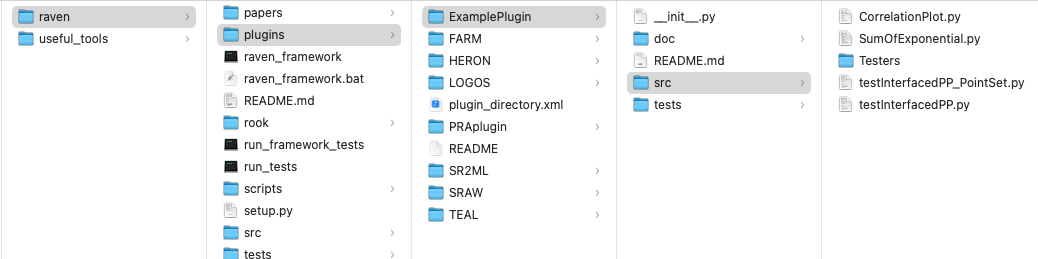
\includegraphics[width=1.0\textwidth]{pics/plugins_location.png}
\caption{Plugins Location}
\label{fig:pluginsLocation}
\end{figure}

\subsection{Plugin Entities}
The procedure of adding a plugin entity for RAVEN is a straightforward process.
The addition of the entity does not require modifying RAVEN itself.
Instead, the developer creates a new Python module inherited from plugin base class that is going to be embedded
in RAVEN at run-time (no need to introduce  hard-coded statements). These RAVEN plugin base
classes are located at \texttt{raven/ravenframework/PluginBaseClasses}:
\begin{lstlisting}[language=bash]
 ExternalModelPluginBase in ExternalModelPluginBase.py
 PlotPlugin in OutStreamPlotPlugin.py
 PostProcessorPluginBase in PostProcessorPluginBase.py
 SupervisedLearningPlugin in SupervisedLearningPlugin.py
\end{lstlisting}
These classes can be loaded as follows in the Python modules created by the plugin developers:
\begin{lstlisting}[language=python, basicstyle=\scriptsize\ttfamily, breaklines=True, columns=fullflexible]
 from ravenframework.PluginBaseClasses.ExternalModelPluginBase import ExternalModelPluginBase
 from ravenframework.PluginBaseClasses.OutStreamPlotPlugin import PlotPlugin
 from ravenframework.PluginBaseClasses.PostProcessorPluginBase import PostProcessorPluginBase
 from ravenframework.PluginBaseClasses.SupervisedLearningPlugin import SupervisedLearningPlugin
 from ravenframework.PluginBaseClasses.CodePluginBase import CodePluginBase

 class NewExternalModelPluginEntity(ExternalModelPluginBase):
   ...

 class NewPlotPluginEntity(PlotPlugin):
   ...

 class NewPostProcessorPluginEntity(PostProcessorPluginBase):
   ...

 class NewROMPluginEntity(SupervisedLearningPlugin):
   ...

 class NewCodePluginEntity(CodePluginBase):
   ...

\end{lstlisting}
The APIs for these classes can be either found in the following sections or directly in the modules themselves.

\subsection{Common Methods for Plugin Entities}
\label{subsec:commonMethods}
\subsubsection{Method: \texttt{getInputSpecification}}
\label{subsubsec:getInputSpecification}
RAVEN uses \texttt{InputData} module to describe data types, check and read XML inputs
(see \url{https://github.com/idaholab/raven/wiki/input-data} for more detailed description).
In order to use this feature, the plugin developers need to load \texttt{InputData} and \texttt{InputTypes}
modules in the developed plugin entity class, i.e.,
\begin{lstlisting}[language=python]
from ravenframework.utils import InputData, InputTypes
\end{lstlisting}
And add a class method called \texttt{getInputSpecification}:
\begin{lstlisting}[language=python, basicstyle=\scriptsize\ttfamily, breaklines=True, columns=fullflexible]
@classmethod
def getInputSpecification(cls):
  """
    Method to get a reference to a class that specifies the input
    data for class cls.
    @ In, None
    @ Out, specs, InputData.ParameterInput, class to use for
      specifying input of cls.
  """
  specs = super().getInputSpecification()
  specs.addParam("xmlAttributeName", param_type=InputTypes.StringType, required=True, default='no-default', descr='')
  subNode = InputData.parameterInputFactory('subnodeName', contentType=InputTypes.StringType, default='no-default', decr='')
  subNode.addParam("xmlSubNodeAttributeName", param_type=InputTypes.StringType, required=True, default='no-default', descr='')
  specs.addSub(subNode)
  return specs
\end{lstlisting}
Since the plugin entities inherit from RAVEN plugin base class, they can get the parent input specification, and use
that as a start (i.e., \texttt{specs = super().getInputSpecification()}).

\subsubsection{Method: \texttt{\_\_init\_\_}}
\label{subsubsec:init}
As the constructor for Python classes, the \texttt{\_\_init\_\_} method should be extended to define
any instance variables used in the plugin class. If no instance variables are used, this may be ommitted.

Any call to \texttt{\_\_init\_\_} must include a call to the parent's constructor, such as
\begin{lstlisting}[language=python]
def __init__(self):
  """ ... """
  super().__init__()
\end{lstlisting}
This assures access to basic RAVEN functionalities required to use the plugin.

\subsubsection{Method: \texttt{handleInput or \_handleInput}}
\label{subsubsec:handleInput}
This API is used by RAVEN to process the input specifications generated by \texttt{getInputSpecification}.
The input to this method is the input specification class instance returned from
\texttt{getInputSpecification}, with \texttt{parseNode} function from this class instance has been already called on the
RAVEN XML node (See \url{https://github.com/idaholab/raven/wiki/input-data} for more detailed description).

\begin{lstlisting}[language=python]
def _handleInput(self, specs):
  """
    Function to handle the parameter input.
    @ In, specs, InputData.ParameterInput, the already-parsed input.
    @ Out, None
  """
  super()._handleInput(specs)
\end{lstlisting}
Depend on the APIs of entities, either \texttt{handleInput or \_handleInput} can be used.
Similar to other methods, any call to \texttt{handleInput or \_handleInput} must include a call to the
paraent's method using \texttt{super()}.

\subsubsection{Method: \texttt{initialize}}
\label{subsubsec:initialize}
The \texttt{initialize} method can be implemented in the plugin entities in order
to initialize some variables needed by it. For example, it can be used to compute a quantity
needed by the \texttt{run} method in \textbf{ExternalModel} plugin. RAVEN is going to call it
at the initialization stage of each \textbf{Step}. RAVEN will communicate, through a set of method
attributes, all the information that are generally needed to perform an initialization:

\begin{itemize}
  \item \texttt{runInfo}, a dictionary containing information regarding how the
  calculation is set up (e.g. number of processors, etc.).
  %
  It contains the following attributes:
  \begin{itemize}
    \item \texttt{DefaultInputFile} -- default input file to use
    \item \texttt{SimulationFiles} -- the xml input file
    \item \texttt{ScriptDir} -- the location of the pbs script interfaces
    \item \texttt{FrameworkDir} -- the directory where the framework is located
    \item \texttt{WorkingDir} -- the directory where the framework should be
    running
    \item \texttt{TempWorkingDir} -- the temporary directory where a simulation
    step is run
    \item \texttt{NumMPI} -- the number of mpi process by run
    \item \texttt{NumThreads} -- number of threads by run
    \item \texttt{numProcByRun} -- total number of core used by one run (number
    of threads by number of mpi)
    \item \texttt{batchSize} -- number of contemporaneous runs
    \item \texttt{ParallelCommand} -- the command that should be used to submit
    jobs in parallel (mpi)
    \item \texttt{numNode} -- number of nodes
    \item \texttt{procByNode} -- number of processors by node
    \item \texttt{totalNumCoresUsed} -- total number of cores used by driver
    \item \texttt{queueingSoftware} -- queueing software name
    \item \texttt{stepName} -- the name of the step currently running
    \item \texttt{precommand} -- added to the front of the command that is run
    \item \texttt{postcommand} -- added after the command that is run
    \item \texttt{delSucLogFiles} -- if a simulation (code run) has not failed,
    delete the relative log file (if True)
    \item \texttt{deleteOutExtension} -- if a simulation (code run) has not
    failed, delete the relative output files with the listed extension (comma
    separated list, for example: `e,r,txt')
    \item \texttt{mode} -- running mode, curently the only mode supported is
      mpi (but custom modes can be created)
    \item \textit{expectedTime} -- how long the complete input is expected to
    run
    \item \textit{logfileBuffer} -- logfile buffer size in bytes
  \end{itemize}
  \item \texttt{inputs}, a list of all the inputs that have been specified in the
  ``Step'' using this model.
  \item \texttt{initDict}, a dictionary with initialization options.
  %
\end{itemize}

\begin{lstlisting}[language=python]
def initialize(self, runInfo, inputs, initDict=None):
  """
    Method to initialize this object before use in each Step
    @ In, runInfo, dict, dictionary of run info
          (e.g. working dir, etc)
    @ In, inputs, list, list of inputs
    @ In, initDict, dict, optional, dictionary with
          initialization options
    @ Out, None
  """
  super().initialize(runInfo, inputs, initDict)
\end{lstlisting}


\subsection{Additional Libraries}
If the plugin requires additional libraries, they can create the \texttt{dependencies.xml} file in
the same manner as RAVEN's dependencies file. Only the libraries that are required by
the plugin but not listed in \texttt{raven/dependencies.xml} are required to be added in the \texttt{pluginName/dependencies.xml}
In this case, libraries will be added like they are for RAVEN
itself, and a check will be performed to assure no base RAVEN (or other plugin) dependencies are
modified.

\subsection{Installing in RAVEN}
Use the installation script in \texttt{raven/scripts/install\_plugins.py}.
\begin{lstlisting}[morekeywords={examplePlugin, pluginInstallation}]
  raven/scripts/install_plugins.py -s /abs/path/to/pluginName
\end{lstlisting}
Replacing \texttt{pluginName} with the path to your plugin and the name of the directory, such as
\texttt{/user/projects/raven/plugins/pluginName}.
Use the absolute path to your new plugin to avoid any navigation problems.
If installing an officially-supported plugin that you do not plan on modifying, the following command
can be run (using TEAL as the example plugin):
\begin{lstlisting}[morekeywords={examplePlugin, TEALInstallation}]
  raven/scripts/install_plugins.py -s TEAL
\end{lstlisting}
Note the path was eliminated. This will initialize (or update) the official plugin in
\texttt{raven/plugins} with the official submoduled version.
To install all officially-supported plugins, the shortcut option \texttt{-a} or \texttt{--all} can be used:
\begin{lstlisting}[morekeywords={examplePlugin, installAllPlugin}]
  raven/scripts/install_plugins.py -a
\end{lstlisting}
At this stage, RAVEN will import all the plugins within that directory and perform some error checking.

This process automatically registers the plugin in the plugin directory, and informs the plugin
about RAVEN %(TODO more notes on this!)

\subsection{Using the Plugin in RAVEN}
Once registered/installed, the new plugin entity (i.e., inherited from ExternalModel, ROM, PostProcessor) can be used in RAVEN input file by
using corresponding RAVEN entity and its \xmlAttr{subType} to load the plugin entity. The \xmlAttr{subType} is defined by your plugin name and your
plugin entity name separated by `.'.
For example, if your plugin external model class is named ``myPluginModel'',
you can access an external model in the RAVEN input as

\begin{lstlisting}[style=XML, morekeywords={usingPlugin}]
<Models>
  ...
  <ExternalModel name='myName' subType='myPluginName.myPluginModel'>
    ...
  </ExternalModel>
  ...
</Models>
\end{lstlisting}

\subsection{Adding Testers}
RAVEN automatically provides a testing harness for automated regression testing. This includes a
variety of \emph{testers}, such as CSV checkers and XML checkers.

If a plugin requires additional testers for regression testing, they can be added to the plugin and
loaded by RAVEN's test harness at testing time.

Any new testers should be added under a folder named \texttt{Testers} in the \texttt{src} directory
of the plugin. For example, for a plugin named \texttt{examplePlugin} and a tester named
\texttt{myNewTester}:
\begin{lstlisting}[morekeywords={examplePlugin,myNewTester}]
  /path/to/examplePlugin/src/Testers/myNewTester.py
\end{lstlisting}
Any discovered testers will be made available to the \texttt{tests} files used by the RAVEN
regression test system; for example:
\begin{lstlisting}[morekeywords={myNewTester}]
[Tests]
  [./aTestForMyPlugin]
    type = myNewTester
    input = my_test_input.xml
    csv = 'TestWorkingDir/results.csv'
  [../]
[]
\end{lstlisting}

For more information on inheriting from and creating new testers, see the RAVEN regression system
documentation.
